\subsection{Mikroprocessor}
\subsubsection{Arduino Mega 2560}
For at kunne opfylde kriterierne sat i kravspecifikationen, har gruppen valgt en Arduino Mega 2560. Denne indeholder 256kb flash memory hvilket gør den mere anvendelig i forhold til UCN boardet, som har 128kb flash memory. I videreudvilking af produktet benyttes et shield, hvilket muliggør anvendelsen af flere digitale pins. Da Ucn boardet ikke er kombatibelt med dette, ses dette som tilstrækkelig grundlag for at benytte Arduino Mega 2560. 
\newline
Mikroprocessoren besidder 54 digitale pins og 14 analog pins der fungerer som in- og output. Derudover har den 4 UART (hardware serial ports) pins som anvedes til at integrere med microproicessorens interface. Pins'ne fungerer i et spændingsintervallet mellem 0-5 V. 
\newline
ATMega2560 er Arduino Mega's processor og har en clock frekvens på 16 MHz. Strømmen tilføres gennem usb, power jack eller gennem pin V_{in} og anbefales en spænding mellem 7-12 V. 
\newline
Mikroprocessoren kan forbindes til computeren ved hjælp af usb, som gør det muligt for de to enheder at kommunikere sammen. Gennem usb forbindelsen kan softwaren overføres fra computeren til den anden enhed. Om nødvendigt kan softwaren genstartes på mikroprocessoren gennem en resetknap, som er monteret på dens PCB.
\newline 
Arduino Mega 2560 har den fordel at være kombatibel med standard bibliotekerne fra Arduino, hvorimod UCN boardet vil kræve at alt softwaren skal bygges fra begyndelsen.

\begin{figure}[h!]
  \centering
  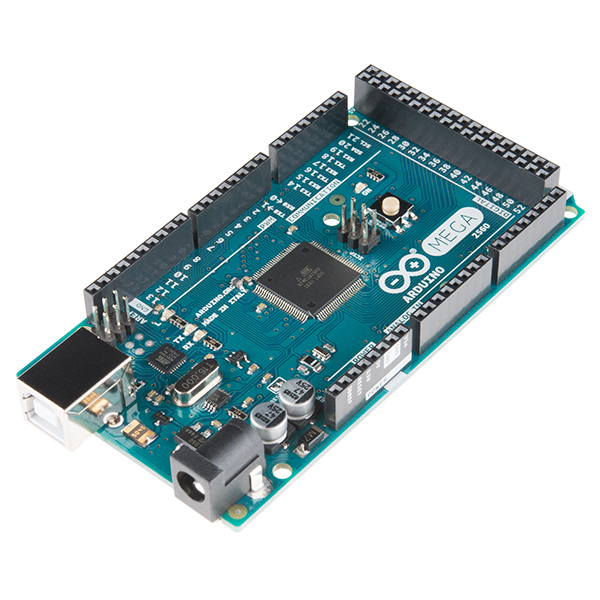
\includegraphics[width=0.7\textwidth]{figures/arduinoMega.jpg}
  \caption{Arduino Mega 2560.}
  \label{tempgraf_eksempel1}
\end{figure} 

\fxnote{fiks billede position}

\newpage



